\documentclass{article}

\usepackage{xcolor}
\usepackage{amsmath,amssymb}
\usepackage{tikz}
%\usepackage{verbatim}
%\usepackage{float}
%\usetikzlibrary{calc}
%\usetikzlibrary{decorations.pathreplacing, arrows.meta}
%\usepackage{amsmath}
%\usepackage{amssymb}
%\usepackage{lmodern}
\usetikzlibrary{decorations.markings}

  
\begin{document}
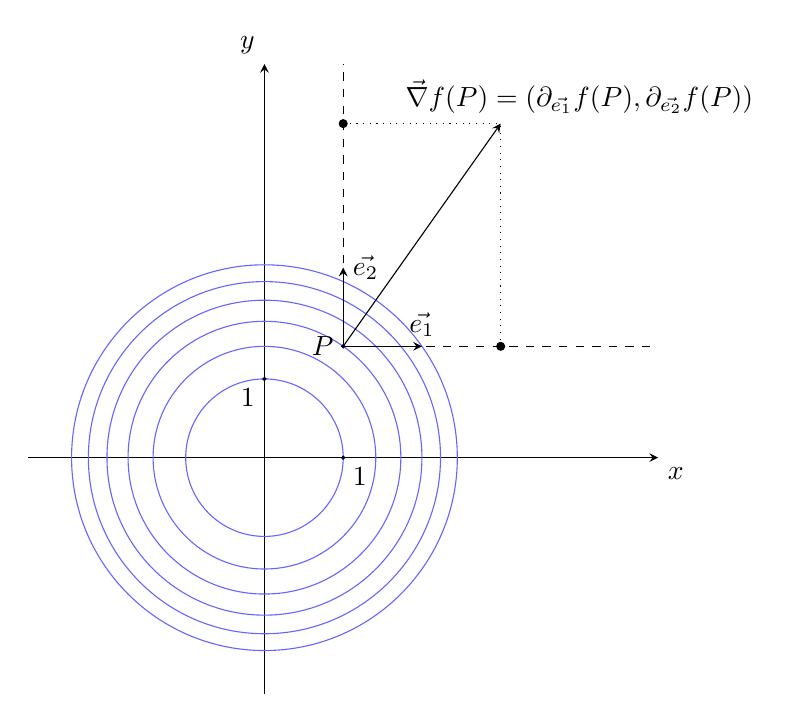
\begin{tikzpicture}[>=stealth]
    %Assen
    %\draw[step=1cm,gray!30,very thin] (-3,-3) grid (5,5);
    \draw [->](0,-3) -- (0,5) node[above left]{$y$};
    \draw [->](-3,0) -- (5,0) node[below right]{$x$};
    %cirkels voor \phi=x^2+y^2
    \draw[blue!60] (0,0) circle (1);
    \draw[blue!60] (0,0) circle (1.7321);
    \draw[blue!60] (0,0) circle (1.4142);
    \draw[blue!60] (0,0) circle (2);
    \draw[blue!60] (0,0) circle (2.2361);
    \draw[blue!60] (0,0) circle (2.4495);
    %coordinaten
    \coordinate (e1) at (1,0);
    \coordinate (e2) at (0,1);
    \coordinate (u1) at (3,1.4142);
    \coordinate (u2) at (1,4.2426);
    \coordinate (P) at (1,1.4142);
    \coordinate (fp) at (4,4.2426);
    \draw[fill=black] (e1) circle(0.02) node[below right] {$1$};
    \draw[fill=black] (e2) circle(0.02) node[below left] {$1$};
    \draw[fill=black] (u1) circle(0.05);
    \draw[fill=black] (u2) circle(0.05);
    \draw[fill=black] (P) circle(0.02) node[left] {$P$};
    \draw [->](1,1.4142) -- (3,4.2426);
    \node[above] at (fp) {$\vec{\nabla} f(P)=(\partial_{\vec{e_1}} f(P),\partial_{\vec{e_2}} f(P))$};
    \draw [->](1,1.4142) -- (2,1.4142) node[above]{$\vec{e_1}$};
    \draw [->](1,1.4142) -- (1,2.4142) node[right]{$\vec{e_2}$};
    \draw[dashed] (1,1.4142) -- (5,1.4142);
    \draw[dashed] (1,1.4142) -- (1,5);
    \draw[dotted] (1,4.2426) -- (3,4.2426);
    \draw[dotted] (3,1.4142) -- (3,4.2426);
    %\node[below] at (u1) {$\partial_{\vec{e_1}} f(P)$};
    %\node[left=0.11cm] at (u2) {$\partial_{\vec{e_2}} f(P)$};
\end{tikzpicture}

\end{document}